\section{Proposed Research}
We propose a prediction-based solution to support efficient and consistent concurrency control. Our approach is based on building a reputation for each transaction using its efficiency rate (i.e., computational cost) and the outcome (i.e., commit or abort). Using these properties transactions are categorized into four categories. The priorities associated with each category impact the transaction's scheduling. Our aim is to prevent cascading rollbacks and inconsistent database state while supporting practical concurrency control. We propose new lock types corresponding to transaction categories. Using these locks transaction scheduler will be able to determine which lock requests to permit. These eventually determine transaction scheduling, delays, and aborts. Our expectation is that prediction-based scheduling will increase both efficiency and consistency.

We identified three research areas in the context of prediction-based scheduling within web service environments that need to be addressed. These are:
\begin{itemize}
    \item transactional correctness within concurrency control
    \item predictions within multi-level secure databases
    \item dynamic reputation for transactions
    % \item prediction-based scheduler within linked databases
\end{itemize}

\subsection{Transactional Correctness}
In this work we aim to develop the theoretical foundation for the prediction-based scheduling. This includes the development of a framework, associated concepts, and technologies. A completely new concurrency control paradigm will be developed in order to elevate particular transactions over others. In this paradigm there are three actions used to determine the course of action for a particular transaction. These three actions either grant, elevate, and decline an transaction to enable concurrent operations and prevent deadlock. By ensuring the transactional correctness within the prediction-based solution, we can then use this foundation to build upon in regards to other research areas. The work discussed in this area is documented in Chapter \ref{chap:prediction_based_scheduler}.

\begin{figure}[h]
\captionsetup{justification=centering}
\centering
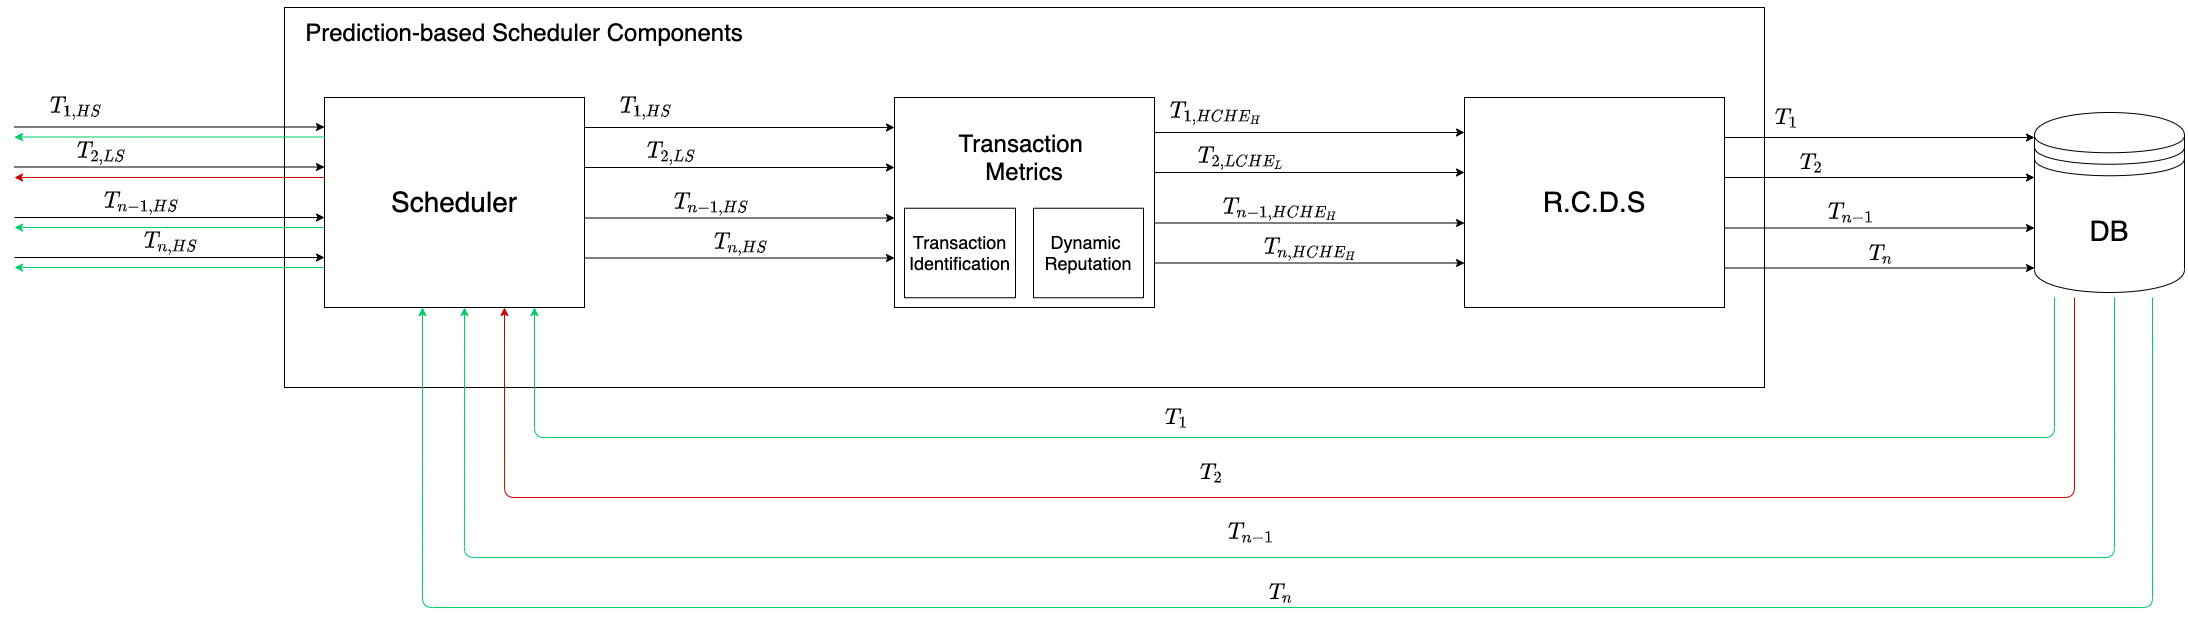
\includegraphics[width=\textwidth]{images/SystemModel_Overall}
\caption{Overall System Model of Prediction-based Scheduler}
\label{fig:system_model_overall}
\end{figure}

\subsection{Multi-level Secure Databases}
After the framework for transactional correctness has been developed (work published in \cite{ravan_ensuring_2020}) within the prediction-based solution we can then begin extending the two-dimensional categorization of the prediction-based scheduler to a three-dimensional categorization for multi-level secure database. The third dimension would include the security classification and allow for a much more robust decision-model. This portion of the overall solution would focus on multi-level secure database systems and covert timing channels. By providing a third dimension to the existing framework we can therefore extend our categorization structure. This allows us to provide a cover story for the timing difference of transactions with differing security classifications. With that cover story in mind we can then provide a solution that elevates high security transactions would the presence of a covert timing channel. The work discussed in this area is documented in Chapter \ref{chap:multi_level_security}.

\subsection{Dynamic Reputation for Transactions}
In both previous sections, the categorization of the transaction is assumed in order to continue forward with the decision model. This section of the proposal would involve the work needed to establish a dynamic reputation management system to allow for dynamic categorization. It would involve building a flyweight for each transaction class that extracts intrinsic transaction attributes from extrinsic attributes. Once a class of transactions are identified we can then use dynamic reputation management to dynamically promote and demote transaction classes throughout the transactional categories. This then allows the system to adapt to its environment dynamically. The work discussed in this area is documented in Chapter \ref{chap:dynamic_reputation}.

% Figure \ref{fig:system_model_overall} displays the system model for the work done for transactional correctness and building a dynamic reputation for transactions.

% \subsection{Snapshot Isolation}
% The third needed to complete the prediction-based solution is the ability to perform snapshot isolation within the different categorizations of transactions. This extension will be for both malicious and lower priority transactions that affect the majority of well-performing transactions. In this work we'll use snapshot isolation to execute certain categorizations of transactions on snapshots of the database in order to prevent the effects of low-performing transactions from affecting all transactions. Once the outcome of a transaction has been determined then the snapshot can either be discarded or merged. With these extensions completed and functioning together effectively, we believe the prediction-based solution will be addressed completely and successfully.

% \subsection{Prediction-based Scheduling within Linked Databases}
% The third and final research area to be addressed is the issue of efficient concurrency control within linked database environments. Currently the Prediction-based solution addresses efficient concurrent transactions within a web-service environment that are contained within a single cluster. This particular area of research will address the problem through the lens of the Prediction-based solution. The difficulty of the problem within this work is adapting the existing framework of correctness built within the Prediction-based solution so that it will scale to linked database systems while preserving its existing capabilities. Figure \ref{fig:system_model_linked_databases} shows the system model for the Prediction-based solution within linked database systems.

% \begin{figure}[h]
% \captionsetup{justification=centering}
% \centering
% \includegraphics[width=\textwidth]{images/LinkedDatabase_SystemModel}
% \caption{Prediction-based Scheduler within Linked Databases}
% \label{fig:system_model_linked_databases}
% \end{figure}

